\documentclass{ecgd-l}

%     If you need symbols beyond the basic set, uncomment this command.
%\usepackage{amssymb}

%     If your article includes graphics, uncomment this command.
\usepackage{graphicx}

%     If the article includes commutative diagrams, ...
%\usepackage[cmtip,all]{xy}

\usepackage{hyperref}

%     Update the information and uncomment if AMS is not the copyright
%     holder.
%\copyrightinfo{2009}{American Mathematical Society}

\newtheorem{theorem}{Theorem}[section]
\newtheorem{lemma}[theorem]{Lemma}

\theoremstyle{definition}
\newtheorem{definition}[theorem]{Definition}
\newtheorem{example}[theorem]{Example}
\newtheorem{xca}[theorem]{Exercise}

\theoremstyle{remark}
\newtheorem{remark}[theorem]{Remark}

\numberwithin{equation}{section}

\newcommand{\G}{\mathbb{G}}
\newcommand{\V}{\mathbb{V}}
\newcommand{\R}{\mathbb{R}}
\newcommand{\nvai}{\infty}
\newcommand{\nvao}{o}

\begin{document}

% \title[short text for running head]{full title}
\title{A Method Of Applying Conformal Transformations Using Geometric Algebra}

%    Only \author and \address are required; other information is
%    optional.  Remove any unused author tags.

%    author one information
% \author[short version for running head]{name for top of paper}
\author{Spencer T. Parkin}
\address{Weber State University\\3848 Harrison Blvd\\Ogden, UT  84408}
\curraddr{}
\email{}
\thanks{}

%    \subjclass is required.
\subjclass[2010]{Primary }

\date{}

\dedicatory{}

%    Abstract is required.
\begin{abstract}
It is shown that any conformal transformation may be applied to a polynomial
of degree $m$
by first converting the polynomial to an $m$-vector taken from a geometric algebra,
applying a versor to that $m$-vector, and then converting the resulting $m$-vector
back into a polynomial.
\end{abstract}

\maketitle

\section{Preliminaries}

For this paper, we assume the reader is already familiar with geometric algebra and the
conformal model of geometric algebra.
(See \cite{Dorst07} for introductory material on geometric algebra.  See \cite{Dorst07,Hestenes01} for material
on conformal geometric algebra.)  Despite what conventions
may be used in other papers on geometric algebra, here we will let the outer product
take precedence over the inner product, and the geometric product take precedence
over the inner and outer products.

As there are different ways of defining the inner product for different purposes, we must
take a moment here to define the inner product used in this paper.  It is as follows.
Among vectors, the inner product is a bilinear form defining the signature of our geometric algebra
which will be given in the next section.  For any vector $v$ and $k$-blade $A$, we define
\begin{equation}\label{equ_def_inner_prod}
v\cdot A = -\sum_{i=1}^k(-1)^i(v\cdot a_i)A_i,
\end{equation}
where here, the $k$-blade $A$ may be factored as $A=\bigwedge_{i=1}^k a_i$,
and for each integer $i\in[1,k]$, we let
\begin{equation*}
A_i=\bigwedge_{\substack{j=1\\j\neq i}}^k a_j.
\end{equation*}
We let $v$ commute with $A$ as
\begin{equation*}
v\cdot A=-(-1)^kA\cdot v.
\end{equation*}
It is sometimes convenient to rewrite equation \eqref{equ_def_inner_prod} as
\begin{equation*}
v\cdot A = (v\cdot a_1)A_1 - (v\cdot A_1)\wedge a_1,
\end{equation*}
which gives a recursive version of the definition.  For the $k$-blade $A$ and
$l$-blade $B$, we define
\begin{equation}\label{equ_A_dot_B}
A\cdot B = \left\{\begin{array}{ll}
A_k\cdot (a_k\cdot B) & \mbox{if $k\leq l$,} \\
(A\cdot b_1)\cdot B_1 & \mbox{if $k\geq l$,}
\end{array}\right.
\end{equation}
where here, the $l$-blade $B$ may be factored as $B=\bigwedge_{i=1}^l b_i$, and for each
integer $i\in[1,k]$, we let
\begin{equation*}
B_i=\bigwedge_{\substack{j=1\\j\neq i}}^l b_j.
\end{equation*}
In the case that $k=l$, either part of the piece-wise function of equation \eqref{equ_A_dot_B} may be used to
evaluate $A\cdot B$.

\section{The Geometric Algebra}

We begin by letting $\{\G_i\}_{i=1}^m$ be a sequence of $m$ Minkowski geometric algebras upon
which the conformal model of $n$-dimensional euclidean space may be imposed.
Each $\G_i$ is the very geometric algebra found in \cite{Hestenes01}.  If $\V_i$ is a vector space
generating $\G_i$, then $\{e_{i,-},e_{i,+}\}\cup\{e_{i,j}\}_{j=1}^n$ is a set of basis
vectors generating $\V_i$, where $\{e_{i,j}\}_{j=1}^n$ is an orthonormal basis
for an $n$-dimensional euclidean space, and where each of $e_{i,-}$ and
$e_{i,+}$, taken from \cite{LiRockwood01}, is given by
\begin{align*}
e_{i,-} &= \frac{1}{2}\nvai_i + \nvao_i, \\
e_{i,+} &= \frac{1}{2}\nvai_i - \nvao_i,
\end{align*}
where here, $\nvao_i$ and $\nvai_i$ are, for each $\G_i$, the familiar null-vectors
representative of the points at origin and infinity, respectively.
With the exception of zero, we consider the sequence of geometric algebras $\{\G_i\}_{i=1}^m$
to be a set of pair-wise disjoint sets.

Taking our cue from the ``mother algebra'' in \cite{DoranHestenes93},
we are now interested in forming the smallest geometric algebra $\G$
containing each $\G_i$ as a geometric sub-algebra.  This geometric
algebra $\G$ is therefore generated by the vector space $\V$, given by
\begin{equation*}
\V=\bigoplus_{i=1}^m \V_i.
\end{equation*}

We now introduce a function $\Psi_{i,j}:\G\to\G$ defined as
\begin{equation*}
\Psi_{i,j}(E) = \left\{\begin{array}{ll}
S_{i,j,1}E(S_{i,j,1})^{-1} & \mbox{if $i\neq j$,} \\
E & \mbox{if $i=j$}\end{array}\right.,
\end{equation*}
where $S_{i,j,k}$ is the constant given by
\begin{equation}\label{equ_S}
S_{i,j,k} = \left(1-(-1)^ke_{i,-}e_{j,-}\right)\left(1+(-1)^ke_{i,+}e_{j,+}\right)\prod_{r=1}^n\left(1+(-1)^ke_{i,r}e_{j,r}\right).
\end{equation}
Take notice that
\begin{equation*}
(S_{i,j,1})^{-1} = 2^{-(n+2)}S_{i,j,0}.
\end{equation*}
Our definition of $\Psi_{i,j}$ is motivated by the fact that for any vector $v_i\in\V_i$ and its
corresponding vector $v_j\in\V_j$, we have
\begin{equation*}
v_j = \Psi_{i,j}(v_i).
\end{equation*}
Being in correspondence, this means that for all integers $k\in[1,n]$,
we have
\begin{equation*}
v_i\cdot e_{i,k}=v_j\cdot e_{j,k},
\end{equation*}
as well as
\begin{equation*}
v_i\cdot\nvao_i = v_j\cdot\nvao_j,
\end{equation*}
and
\begin{equation*}
v_i\cdot\nvai_i = v_j\cdot\nvai_j.
\end{equation*}
Notice that $\Psi_{i,j}(v_j)=-v_i$.
For any vector $v\not\in\V_i$ and $v\not\in\V_j$, the function $\Psi_{i,j}$ leaves $v$ invariant.

If it could be shown that $S_{i,j,1}$ in equation \eqref{equ_S} is a versor of $\G$,
we could then conclude that $\Psi_{i,j}$ is an outermorphism.
(See \cite{Hestenes91} for a definition of outermorphism.)  Though no such
proof will be given here, we will be able to show that $\Psi_{i,j}$ is indeed
an outermorphism.  To that end, it suffices to show that
for any two vectors $a,b\in\V$, we have
\begin{equation}\label{equ_inner_prod_add_psi}
a\cdot b = \Psi_{i,j}(a)\cdot \Psi_{i,j}(b).
\end{equation}
To see this, begin by rewriting $a$ and $b$ as
$a = \sum_{k=1}^m a_k$ and $b = \sum_{k=1}^m b_k$,
where for each pair $(a_k,b_k)$, we have $a_k,b_k\in\V_k$.  We then have
\begin{equation*}
a\cdot b=\sum_{k=1}^m a_k\cdot b_k,
\end{equation*}
where we can make the observation that for any integer $k\in[1,m]$, we have
\begin{equation*}
a_k\cdot b_k = \Psi_{i,j}(a_k)\cdot\Psi_{i,j}(b_k).
\end{equation*}
We now simply see that
\begin{equation*}
\Psi_{i,j}(a)\cdot\Psi_{i,j}(b)=\sum_{k=1}^m\Psi_{i,j}(a_k)\cdot\Psi_{i,j}(b_k)
\end{equation*}
to complete the proof.

Equation \eqref{equ_inner_prod_add_psi} can now be applied in a proof
that $\Psi_{i,j}$ preserves the outer product.
\begin{align*}
\Psi_{i,j}(a\wedge b) &= \Psi_{i,j}(ab - a\cdot b) \\
 &= \Psi_{i,j}(ab) - \Psi_{i,j}(a\cdot b) \\
 &= \Psi_{i,j}(a)\Psi_{i,j}(b) - a\cdot b \\
 &= \Psi_{i,j}(a)\Psi_{i,j}(b) - \Psi_{i,j}(a)\cdot\Psi_{i,j}(b) \\
 &= \Psi_{i,j}(a)\wedge\Psi_{i,j}(b).
\end{align*}
It is not too difficult to generalize this proof to blades of arbitrary grade.

\section{Geometric Representation}

Having now set forth our geometric algebra $\G$, we're ready to discuss
geometric representation.
Letting $\R^n_j$ denote the $n$-dimensional euclidean vector sub-space
of $\V_j$, our geometric representation scheme is to let a geometry be the
set of all points $x_1\in\R^n_1$, such that
\begin{equation}\label{equ_rep_geo}
\bigwedge_{j=1}^m p_j(x_1)\cdot A=0,
\end{equation}
where $A$ is an $m$-vector (not necessarily an $m$-blade) of $\G$, and
where the function $p_j:\R^n_1\to\V_j$, reminding us of the principle  mapping found in \cite{Hestenes01}, is defined as
\begin{align*}
p_j(x_1)&=\Psi_{1,j}\left(\nvao_1+x_1+\frac{1}{2}x_1^2\nvai_1\right) \\
 &= \nvao_j + x_j + \frac{1}{2}x_j^2\nvai_j,
\end{align*}
where $x_j\in\R^n_j$.
Here, it is the $m$-vector $A$ that serves as the representative of our geometry.
It is not hard to see that the point-set generated by $A$ through equation \eqref{equ_rep_geo}
is simply the zero set of a polynomial of degree at most $2m$.\footnote{An algebraic
set is the zero set of one or more polynomial functions.  It can be shown that such sets may be represented by
the blades of a geometric algebra, but the geometric representation scheme of this paper is restricted to those sets
that are the zero set of one and only one polynomial function.}

For any polynomial of degree $r$ with $m<r\leq 2m$, there does not necessarily exist an $m$-vector $A$ representative of its zero set in terms of the definition just given by
equation \eqref{equ_rep_geo}.  For all polynomials of degree $r$ with $0\leq r\leq m$,
however,
there does exist such an $m$-vector $A$.  Taking advantage of the linearity of the inner product,
it suffices to show that this is the case for every monomial of such a degree.  Indeed, the $m$-vector
$A$, (in this case an $m$-blade), is given by
\begin{equation*}
A = \lambda\bigwedge_{j=1}^r a_j\wedge\bigwedge_{j=r+1}^m\nvai_j,
\end{equation*}
where $\lambda\in\R$ is a scalar, $\{a_j\}_{j=1}^r$ is a set of $r$ vectors with
each $a_j\in\R^n_j$,
and the product $\bigwedge_{j=1}^r a_j$ is one in the case that $r=0$.
To see this, let $x_j=\Psi_{1,j}(x_1)$ and write
\begin{align*}
\bigwedge_{j=1}^m p_j(x_1)\cdot A
 &= \bigwedge_{j=1}^m\left(\nvao_j+x_j+\frac{1}{2}x_j^2\nvai_j\right)\cdot A \\
 &= \bigwedge_{j=1}^r x_j\wedge\bigwedge_{j=r+1}^m\nvao_j\cdot A \\
 &= \pm\lambda\bigwedge_{i=1}^r x_j \cdot\bigwedge_{i=1}^r a_j \\
 &= \pm\lambda\prod_{i=1}^r x_j\cdot a_j,
\end{align*}
which shows that for an appropriate choice of the vectors in $\{a_j\}_{j=1}^r$,
and that of $\lambda$, we can formulate $A$ as being representative of any monomial in $n$
independent variables $\{x_1\cdot e_{1,j}\}_{j=1}^n$.  With some effort,
the sign can be deduced as a function of $m$ and $r$, but this distracts us
from the point being made here.

It is not difficult to convert between polynomial functions and $m$-vectors $A$
of our geometric algebra $\G$.  That is, not difficult if we are using a computer
algebra system.  We'll no doubt want to make further
use of such a system in the section to follow.  It should also be mentioned
that there are often nice conversions between $m$-vectors and vector-based
equations, each of who's solution sets are the geometries in question.  See, for example,
the vector-based equations for quadric surfaces found in \cite{Miller87}.

\section{Applying Conformal Transformations To Geometries}

\begin{figure}
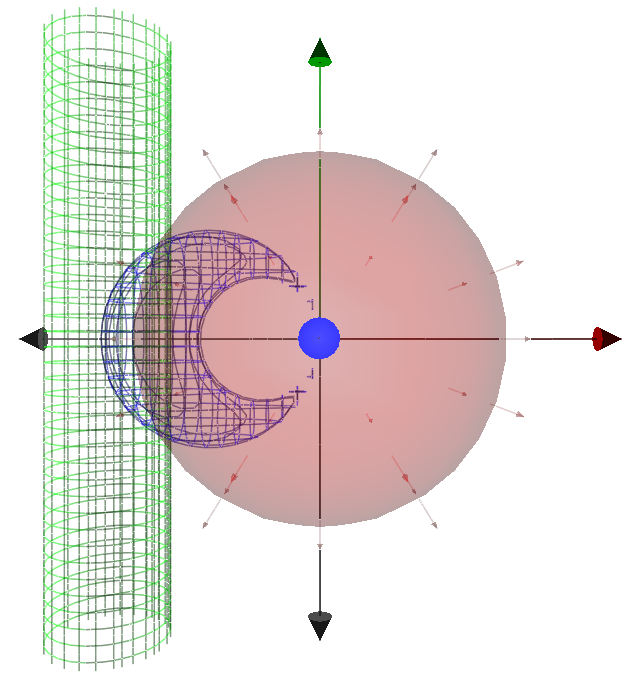
\includegraphics[scale=0.3]{InvertCylinderInSphere}
\caption{The inversion of a cylinder in a sphere.  Traces in various planes were
used to render the cylinder and its inversion.}
\label{fig_invert_cylinder_in_sphere}
\end{figure}
We now come to the main result of this paper, which is to show
that the conformal transformations are easily applicable to any geometry
that may be represented as an $m$-vector by equation \eqref{equ_rep_geo}.
We simply observe that if $V_1\in\G_1$ is a versor representative
of a conformal transformation, (those that can be found in \cite{Dorst07,LiRockwood01}),
then, letting $V_j=\Psi_{1,j}(V_1)$, the desired
geometry is given by the set of all points $x_1\in\R^n_1$, such that
\begin{equation*}
\bigwedge_{j=1}^m V_j^{-1} p_j(x_1) V_j\cdot A=0.
\end{equation*}
It will not be hard to show that the $m$-vector $A'$ representative
of this very set of points by equation \eqref{equ_rep_geo} is given by
\begin{equation*}
A' = WAW^{-1},
\end{equation*}
where the versor $W$ is given by
\begin{equation*}
W = \prod_{j=1}^m V_j.
\end{equation*}
Taking advantage of the linearity of the inner product once again,
we need only prove our main result in the case that $A$ is an $m$-blade.
Let $\{a_j\}_{j=1}^m\subset \V$ be a set $m$ vectors, such that
\begin{equation*}
A = \bigwedge_{j=1}^m a_j.
\end{equation*}
We then have
\begin{align}
\bigwedge_{j=1}^m V_j^{-1}p_j(x_1)V_j\cdot\bigwedge_{j=1}^m a_j &=
\prod_{j=1}^m V_j^{-1}p_j(x_1)V_j\cdot a_j\nonumber \\
 &= \prod_{j=1}^m p_j(x_1)\cdot V_ja_jV_j^{-1}\nonumber \\
&= \bigwedge_{j=1}^m p_j(x_1)\cdot\bigwedge_{j=1}^m V_ja_jV_j^{-1}\nonumber \\
&= \bigwedge_{j=1}^m p_j(x_1)\cdot\bigwedge_{j=1}^m Wa_jW^{-1}\nonumber \\
&= \bigwedge_{j=1}^m p_j(x_1)\cdot WAW^{-1}.\nonumber
\end{align}
This completes the proof.
We can now convert $A'$ into a polynomial equation, which
may be a more usable form than that of an $m$-vector.

In the course of this research, theory was put into practice, and a computer algebra
system with visualization capabilities was implemented and used to generate
Figure~\ref{fig_invert_cylinder_in_sphere}.

In the case of Figure~\ref{fig_invert_cylinder_in_sphere}, we need only
have $m=2$.  The following computer code, consumed by the research
software, illustrates how the figure was generated.
%\begin{samepage}
\begin{center}
{\tiny
\begin{verbatim}

/*
 * Calculate the surface that is the
 * inversion of a cylinder in a sphere.
 */
do
(
    /* Make the cylinder. */
    v = e2, c = -7*e1, r = 2,
    cylinder = Omega - v^bar(v) + 2*c*nib + (c.c - r*r)*ni^nib,
    bind_quadric(cylinder),
    geo_color(cylinder,0,1,0),
	
    /* Make the sphere. */
    c = 0, r = 6,
    sphere = no + c + 0.5*(c.c - r*r)*ni,
    bind_dual_sphere(sphere),
    geo_color(sphere,1,0,0,0.2),
	
    /* Make the inversion of the cylinder in the sphere. */
    V = sphere*bar(sphere),
    inversion = V*cylinder*V~,
    bind_conformal_quartic(inversion),
    geo_color(inversion,0,0,1),
)

\end{verbatim}
}
\end{center}
%\end{samepage}

Here, the ``bar'' function takes the place of $\Psi_{1,2}$, and
the constant $\Omega$ is defined as
\begin{equation*}
\Omega = \sum_{j=1}^n e_{1,j}\wedge e_{2,j}.
\end{equation*}
The ``bind\_*'' functions create and bind a piece of computer code
to the given element that is responsible
for interpreting that element under the named definition.
While the sphere element is interpreted as a dual sphere of the conformal model
of geometric algebra in the usual manner, the cylindrical and inverted
surfaces are interpreted under the definition given earlier using
equation \eqref{equ_rep_geo}.\footnote{The research software
can be found at \url{https://github.com/spencerparkin/GAVisTool}.}

\section{Closing Remarks}

\bibliographystyle{amsplain}
\bibliography{Parkin_AMethodOfApplyingConformalTransformationsUsingGA}

\end{document}